\section{Black formula}\lesson{18}{17/04/2020}
The B\&S formula gives the price of a call option on an asset. The purpose of this section is to derive the Black formula for the price of call options on a \emph{futures} or \emph{forward contract}.\\

\subsection{Forward contracts} % Hull ch.2
Recall the main features of the forward contract:
\begin{itemize}
    \item it gives us the obligation to buy the asset at a fixed price $K$ which is fixed at the signature date;
    \item the payoff is $(S_T-K)$;
    \item the strike $K$ is such that at the signature time the value of the contract is zero (it is cost-less to enter in a forward contract). Furthermore, we can introduce the notion of \emph{forward price} $K(t,T)$, which is the strike price decided at time $t$ such that the value of the ``new contract" starting at time $t$ is zero. In other words, it represents an ``updated baricenter";
    \item using the absence of arbitrage, we found that if the interest rate is constant then
    \begin{equation}
        K(0,T) = S(0)e^{rT} \qquad\Rightarrow\qquad K(t,T) = S(t)e^{r(T-t)}.
    \end{equation}
    If the interest rate is stochastic we have to consider a change of numéraire.
    \item if the strike $K(0,T)=K$ is the fair one, the price is given by:
    \begin{equation}\label{pr03}
        price_t(\pay_{[0,T]}) =
        \begin{cases}
        0 & t=0 \\
        \expect_t\left[e^{-\int_t^T r_s\,\dd s}(S(T)-K(0,T))\right] & 0<t<T \\
        S(T)-K(0,T) & t=T
        \end{cases}
    \end{equation}
    Let's compute the expected value in \eqref{pr03} for $0<t<T$:
    \begin{align*}
        \eqref{pr03} &= e^{-\int_t^T r_s\,\dd s}\expect_t\left[e^{-\int_0^t r_s\,\dd s}S(T)\right] - K(0,T)B(t,T) \\
        \overset{(a)}&{=}
        \cancel{e^{-\int_0^t r_s\,\dd s}}\cancel{e^{-\int_0^t r_s\,\dd s}}S(t) - K(0,T)B(t,T) \\
        &=
        S(t) - K(0,T)B(t,T)
    \end{align*}
    where in (a) we used the fact that the discounted asset $S(t)e^{-\int_0^t r_s\,\dd s}$ is a true $\Qmeas$-martingale. \\
    If the interest rate is flat, $r_t = r$ $\forall t$, we have:
    \begin{align}\label{eq4}
        price_t(S(T)-K(0,T)) = S(t) - K(0,T)e^{-r(T-t)} \gtrless 0
    \end{align}
    which can be positive or negative. Introducing the expression of the forward strike at time $t=0$,
    \begin{equation*}
        K(0,T) = S(0)e^{rT},
    \end{equation*}
    we can rewrite \eqref{eq4} as
    \begin{align}
        \label{eq1}
        price_t(S(T)-K(0,T)) &= S(t) - K(0,T)e^{-r(T-t)} \\
        &=
        \notag S(t) - S(0)e^{rT}e^{-r(T-t)} \\
        &=
        S(t) - S(0)e^{rt} \label{eq2}
    \end{align}
    Eq. \eqref{eq1} is a \emph{forward looking} expression, in the sense that we look for the correct price to exchange with the underlying at time $T$, we discount it and we compare this with the current realization of the underlying $S(t)$. Eq. \eqref{eq2} is a \emph{backward looking} expression, in the sense that the value of the forward contract is positive or negative according to the comparison between the current value of the underlying $S(t)$ and the capitalization of the initial value $S(0)$.
\end{itemize}

\subsection{Futures contracts}
Futures contracts are a particular type of forward contracts in which the counterparts ``do not know/trust each other". If the two counterparts agree to trade an asset in the future for a certain price, there are obvious risks. One of the investors may regret the deal and try to back out. Alternatively, the investor simply may not have the financial resources to honor the agreement. One of the key roles of the exchange is to organize trading so that contract defaults are avoided. This is where futures contracts and margin accounts come in.\\
Instead of signing the contract at time $t=0$ and hope that at time $T$ our counterpart will deliver the corresponding payoff (which can be positive or negative), we require it to deposit funds in a \emph{margin account}. The amount that must be deposited at the time the contract is entered into is known as the \emph{initial margin} and, at the end of each trading day, the margin account is adjusted to reflect the investor's gain or loss $S(t)\gtrless K$. This practice is referred to as \emph{daily settlement} or \emph{marking to market}.
\begin{figure}[ht]
    \centering
    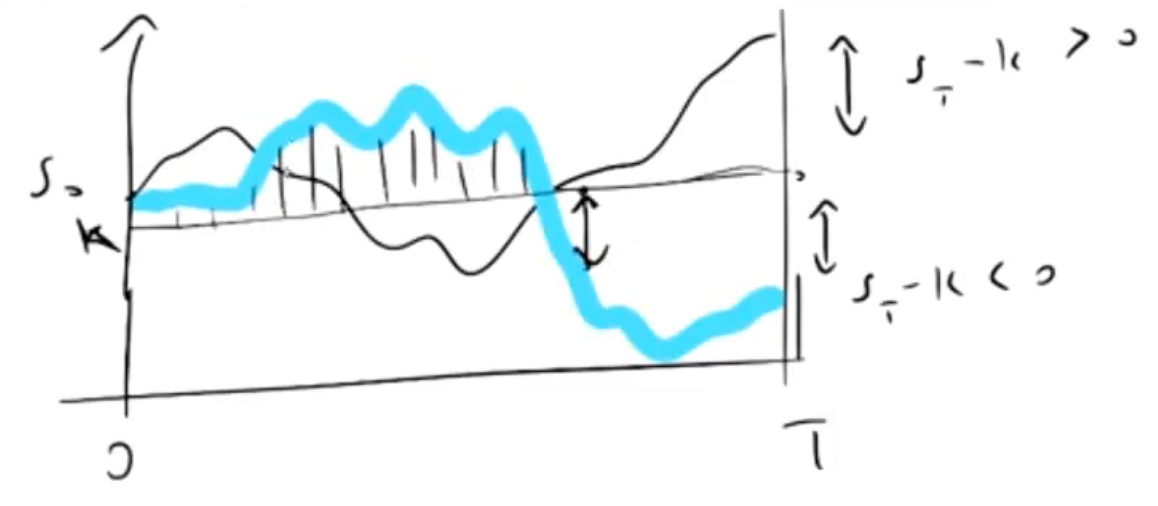
\includegraphics[scale=0.27]{fig/tmp/fig31.png}
    \caption{Futures contracts.}
    \label{fig:futures}
\end{figure}
\newline The investor is entitled to withdraw any balance in the margin account in excess of the initial margin. To ensure that the balance in the margin account never becomes negative a \emph{maintenance margin}, which is somewhat lower than the initial margin, is set. If the balance in the margin account falls below the maintenance margin, the investor receives a \emph{margin call} and is expected to top up the margin account to the initial margin level by the end of the next day. The extra funds deposited are known as \emph{variation margin}. If the investor does not provide the variation margin, the broker closes out the position\footnote{See \cite{hull}, section 2.4.}.\\
\\
Here we will consider a simplified marking to market framework in which we make the following assumptions:
\begin{itemize}
    \item the market to market is on the whole value of the contract, in such a way that if the payoff of the futures at time $T$ is $S(T)-F(0,T)$, then:
    \begin{equation*}
        price_t(\fut) \equiv 0 \quad\forall t
    \end{equation*} % fine parte 1
    \item for all $t$ there is a quoted strike price $F(t,T)$ called \emph{strike price} which makes zero the value of the contract. This means that in the time interval $(s,t]$ the holder of a futures receives the dividend $F(t,T) - F(s,T)$.\\
    For example, if there is a shock in the market so that $F(t,T) - F(s,T) < 0$, the long position has to pay this difference (margin call).
    \item The convergence condition
    \begin{equation}
        F(T,T) = S(T)
    \end{equation}
    holds.
    \begin{figure}[h]
        \centering
        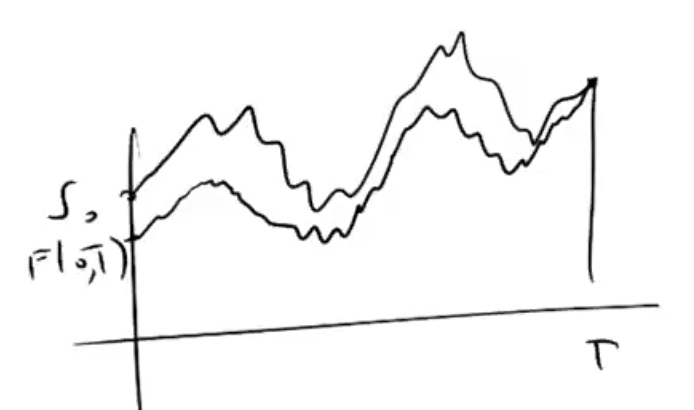
\includegraphics[scale=0.32]{fig/tmp/fig32.png}
        \caption{Converge condition of the underlying}
        \label{fig:concond}
    \end{figure}
\end{itemize}
In summary:
\begin{itemize}
    \item $price_t = 0$ $\forall t\le T$ (this plays the role of $S_t$);
    \item The dividend is equal to the futures price: $D(t)=F(t,T)$;
    \item $F(T,T)=S(T)$ (boundary condition).
\end{itemize}
From Section \ref{B&Swithdividends} we know that in presence of dividends the discounted asset is not a martingale, but the normalized gain process
\begin{align}
    S(t)e^{-\int_0^t r_s\,\dd s} + \int_0^t e^{-\int_0^s r_u\,\dd u}\dd D
\end{align}
is a $\Qmeas$-martingale. But in futures contracts
\begin{equation*}
    S(t) \leftrightarrow price_t \equiv 0, \quad \dd D \leftrightarrow \dd F
\end{equation*}
so we are left with:
\begin{align}\label{it}
    \int_0^t e^{-\int_0^s r_u\,\dd u}\,\dd F_s \overset{(a)}{=} \int_0^t h_s\,\dd W_s^{\Qmeas}
\end{align}
where in (a) we used the representation theorem for continuous (Brownian) martingales, which allows us to write the integral as a Brownian integral introducing an appropriate adapted process $h_s$. Writing \eqref{it} in its infinitesimal form we have:
\begin{equation}
    e^{-\int_0^s r_u\,\dd u}\,\dd F_t = h_s\,\dd W_s^{\Qmeas} \qquad\Rightarrow\qquad \dd F(t,T) = \left(e^{\int_0^s r_u\,\dd u}h_t\right)\,\dd W_s^{\Qmeas}.
\end{equation}
In other words, we have that $F(t,T)$ is a $\Qmeas$-martingale. So, by martingality, the futures' price at time $t$ is given by:
\begin{equation}\label{futurespriceattimet}
    F(t,T) = \expect_t[F(T,T)] = \expect_t[S(T)] = \expect[S(T)|\mathcal{F}_t]
\end{equation}
Recall that for the forward contract we found that:
\begin{equation}
    K(t,T) = \expect_t\left[\dfrac{e^{-\int_t^T r_s\,\dd s}S(T)}{B(t,T)}\right] = \mathbb{E}^{\Qmeas^T}_t[S(T)]
\end{equation}
So forward price and futures price are both the expected value of the underlying at time $T$ but they are computed under different probability measures (forward risk neutral measure and risk neutral measure). \\
Forward price and futures are the same if the two probability measures are the same. For example, this is true when the interest rate is deterministic.

\subsection{Black formula} % Bjork pag. 108
The Black formula gives the price of a call on a futures (on $S$). Here we assume that the underlying evolves according to the B\&S dynamics with constant interest rate, $r_t \equiv r$. In this framework, if we denote with $X$ the strike price of the call and we choose $T_1 > T$ as maturity of the call option, the payoff is
\begin{equation}
    \pay_T = (F(T,T_1) - X)^+ + \underbrace{\pay_T(\text{long position on the futures})}_{=0}
\end{equation}
In other words, we have a contract on a contract, which is called \emph{compounded option}. \\
Using eq. \eqref{futurespriceattimet} we can write:
\begin{align}
    \notag (F(T,T_1) - X)^+ &= \left(S(T)e^{r(T_1-T)} - X\right)^+ \\
    &=
    e^{r(T_1-T)}\left(S(T)-Xe^{-r(T_1-T)}\right)^+
\end{align}
Recall that according to the B\&S formula the price of a call is given by:
\begin{equation*}
    price_t(\call) = S(t)\Phi(d_1)-Ke^{-r(T-t)}\Phi(d_2)
\end{equation*}
In this case
\begin{equation*}
    K = Xe^{-r(T_1-T)}, \qquad S(t) = F(t,T_1)e^{-r(T_1-t)}
\end{equation*}
so we have:
\begin{align*}
    price_t(\call(\fut)) &= e^{r(T_1-T)} \left(S(t)\Phi(d_1)-e^{-r(T-t)}Xe^{-r(T_1-T)}\Phi(d_2)\right) \\
    &=
    e^{r(T_1-T)}S(t)\Phi(d_1)-e^{-r(T-t)}Xe\Phi(d_2) \\
    &=
    e^{-r(T-t)}\left(\underbrace{S(t)e^{-r(T_1-t)}}_{F(t,T_1)}\Phi(d_1) - X\Phi(d_2)\right)
\end{align*}
We end up with the so called \emph{Black formula}:
\begin{equation}
    price_t(\call(\fut)) = e^{-r(T-t)}\left(F(t,T_1)\Phi(d_1) - X\Phi(d_2)\right)
\end{equation}
where in this case:
\begin{equation}
    d_1 = \dfrac{\ln\frac{F(t,T_1)}{X}+\frac{1}{2}\sigma^2(T-t)}{\sigma\sqrt{T-t}}, \qquad d_2 = d_1 - \sigma\sqrt{T-t}. %giusto
\end{equation}
